\documentclass{standalone}
\usepackage[utf8]{inputenc}
\usepackage{tikz}
\usepackage{verbatim}


\usepackage{pgfplots}
\DeclareUnicodeCharacter{2212}{−}
\usepgfplotslibrary{groupplots,dateplot}
\usetikzlibrary{patterns,shapes.arrows}
\usetikzlibrary {fit} 
\usetikzlibrary{shapes.geometric,positioning}
\usetikzlibrary{bending}
\pgfplotsset{compat=1.16}

\begin{document}


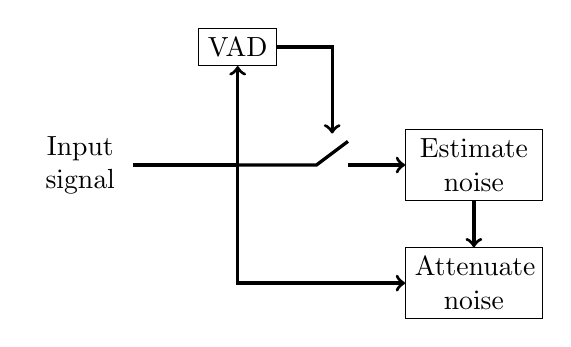
\begin{tikzpicture}
    \node at (0,0) (in) {\parbox{1.1cm}{\centering Input signal}};
    \node[draw] at (2,1.5) (vad) {VAD};
    \node[draw] at (5,0) (est) {\parbox{1.5cm}{\centering Estimate noise}};
    \node[draw] at (5,-1.5) (enh) {\parbox{1.5cm}{\centering Attenuate noise}};
    \draw[->,very thick] (in) -- (2,0) -- (2,-1.5) -- (enh);
    \draw[->,very thick] (in) -- (2,0) -- (vad);
    \draw[->,very thick] (est) -- (enh);
    \draw[very thick] (in) -- (3,0) -- (3.4,0.3);
    \draw[very thick,->] (3.4,0) -- (est);
    \draw[->,very thick] (vad) -- (3.2,1.5) -- (3.2,0.4);
\end{tikzpicture}

\end{document}
